

\tikzset{every picture/.style={line width=0.75pt}} %set default line width to 0.75pt        

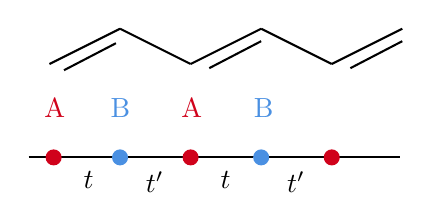
\begin{tikzpicture}[x=0.75pt,y=0.75pt,yscale=-1,xscale=1]
%uncomment if require: \path (0,300); %set diagram left start at 0, and has height of 300

%Straight Lines [id:da9956235879402113] 
\draw    (100,101) -- (134,84) ;
%Straight Lines [id:da7247828675996284] 
\draw    (202,84) -- (168,101) ;
%Straight Lines [id:da5773329935549767] 
\draw    (202,84) -- (236,101) ;
%Straight Lines [id:da3206012026384706] 
\draw    (168,101) -- (144.4,89.2) -- (134,84) ;
%Straight Lines [id:da6366740347566855] 
\draw    (236,101) -- (270,84) ;
%Straight Lines [id:da9111075840879808] 
\draw    (107,104) -- (132,91) ;
%Straight Lines [id:da5940492749723987] 
\draw    (177,103) -- (202,90) ;
%Straight Lines [id:da21751025441510952] 
\draw    (245,103) -- (270,90) ;
%Straight Lines [id:da7004634811978112] 
\draw    (90,146) -- (269,146) ;
%Straight Lines [id:da7336134345483176] 
\draw [color={rgb, 255:red, 208; green, 2; blue, 27 }  ,draw opacity=1 ]   (102,146) ;
\draw [shift={(102,146)}, rotate = 0] [color={rgb, 255:red, 208; green, 2; blue, 27 }  ,draw opacity=1 ][fill={rgb, 255:red, 208; green, 2; blue, 27 }  ,fill opacity=1 ][line width=0.75]      (0, 0) circle [x radius= 3.35, y radius= 3.35]   ;
%Straight Lines [id:da5304413655428435] 
\draw [color={rgb, 255:red, 74; green, 144; blue, 226 }  ,draw opacity=1 ]   (134,146) ;
\draw [shift={(134,146)}, rotate = 0] [color={rgb, 255:red, 74; green, 144; blue, 226 }  ,draw opacity=1 ][fill={rgb, 255:red, 74; green, 144; blue, 226 }  ,fill opacity=1 ][line width=0.75]      (0, 0) circle [x radius= 3.35, y radius= 3.35]   ;
%Straight Lines [id:da016904275323671447] 
\draw [color={rgb, 255:red, 208; green, 2; blue, 27 }  ,draw opacity=1 ]   (168,146) ;
\draw [shift={(168,146)}, rotate = 0] [color={rgb, 255:red, 208; green, 2; blue, 27 }  ,draw opacity=1 ][fill={rgb, 255:red, 208; green, 2; blue, 27 }  ,fill opacity=1 ][line width=0.75]      (0, 0) circle [x radius= 3.35, y radius= 3.35]   ;
%Straight Lines [id:da27782244408746837] 
\draw [color={rgb, 255:red, 74; green, 144; blue, 226 }  ,draw opacity=1 ]   (202,146) ;
\draw [shift={(202,146)}, rotate = 0] [color={rgb, 255:red, 74; green, 144; blue, 226 }  ,draw opacity=1 ][fill={rgb, 255:red, 74; green, 144; blue, 226 }  ,fill opacity=1 ][line width=0.75]      (0, 0) circle [x radius= 3.35, y radius= 3.35]   ;
%Straight Lines [id:da6527169495554346] 
\draw [color={rgb, 255:red, 208; green, 2; blue, 27 }  ,draw opacity=1 ]   (236,146) ;
\draw [shift={(236,146)}, rotate = 0] [color={rgb, 255:red, 208; green, 2; blue, 27 }  ,draw opacity=1 ][fill={rgb, 255:red, 208; green, 2; blue, 27 }  ,fill opacity=1 ][line width=0.75]      (0, 0) circle [x radius= 3.35, y radius= 3.35]   ;

% Text Node
\draw (115,151.4) node [anchor=north west][inner sep=0.75pt]    {$t$};
% Text Node
\draw (145,151.4) node [anchor=north west][inner sep=0.75pt]    {$t'$};
% Text Node
\draw (181,151.4) node [anchor=north west][inner sep=0.75pt]    {$t$};
% Text Node
\draw (213,151.4) node [anchor=north west][inner sep=0.75pt]    {$t'$};
% Text Node
\draw (96,116) node [anchor=north west][inner sep=0.75pt]  [color={rgb, 255:red, 208; green, 2; blue, 27 }  ,opacity=1 ] [align=left] {A};
% Text Node
\draw (162,116) node [anchor=north west][inner sep=0.75pt]  [color={rgb, 255:red, 208; green, 2; blue, 27 }  ,opacity=1 ] [align=left] {A};
% Text Node
\draw (128,116) node [anchor=north west][inner sep=0.75pt]  [color={rgb, 255:red, 74; green, 144; blue, 226 }  ,opacity=1 ] [align=left] {B};
% Text Node
\draw (197,116) node [anchor=north west][inner sep=0.75pt]  [color={rgb, 255:red, 74; green, 144; blue, 226 }  ,opacity=1 ] [align=left] {B};


\end{tikzpicture}
